\documentclass[12pt, preprint]{aastex}

\usepackage{subfigure}
\usepackage{color}
\usepackage{hyperref}
\usepackage{url}
\usepackage{natbib}
\usepackage{amsmath}

\newcommand{\project}[1]{\textsl{#1}}
\newcommand{\cpm}{\project{CPM}}
\newcommand{\cpmdiff}{\project{CPM Difference Imaging}}
\newcommand{\class}{\project{the classical difference imaging}}
\newcommand{\kepler}{\project{Kepler}}
\newcommand{\KTCZ}{\project{K2 Campaign 0}}
\newcommand{\KTCN}{\project{K2 Campaign 9}}
\newcommand{\epic}{\project{EPIC}}
\newcommand{\todo}[1]{\textbf{#1}}
\newcommand{\set}[1]{\mathcal{#1}}

\graphicspath{{figures/}}

\bibliographystyle{apj}
\definecolor{linkcolor}{rgb}{0,0,0.5}
\hypersetup{colorlinks=true,linkcolor=linkcolor,citecolor=linkcolor,
            filecolor=linkcolor,urlcolor=linkcolor}

\begin{document}

\title{A pixel-level model for event discovery in time-domain imaging}
\author{%
  Dun~Wang\altaffilmark{\ref{CCPP},\ref{email}},
  David~W.~Hogg\altaffilmark{\ref{CCPP},\ref{CDS},\ref{MPIA},\ref{FI}},
  Daniel~Foreman-Mackey\altaffilmark{\ref{UW},\ref{SF}}
  Bernhard~Sch\"olkopf\altaffilmark{\ref{MPIIS}}
  }
\newcounter{address}
\setcounter{address}{1}
\altaffiltext{\theaddress}{\stepcounter{address}\label{CCPP}%
  Center for Cosmology and Particle Physics, Department of Physics, New York University}
\altaffiltext{\theaddress}{\stepcounter{address}\label{CDS}%
  Center for Data Science, New York University}
\altaffiltext{\theaddress}{\stepcounter{address}\label{MPIA}%
  Max-Planck-Institut f\"ur Astronomie, Heidelberg, Germany}
\altaffiltext{\theaddress}{\stepcounter{address}\label{email}%
  To whom correspondence should be addressed; \texttt{<dun.wang@nyu.edu>}.}
\altaffiltext{\theaddress}{\stepcounter{address}\label{UW}%
 Astronomy Department, University of Washington, Seattle, WA 98195}
\altaffiltext{\theaddress}{\stepcounter{address}\label{SF}%
Sagan Fellow}
\altaffiltext{\theaddress}{\stepcounter{address}\label{MPIIS}%
  Max-Planck-Institut f\"ur Intelligente Systeme, T\"ubingen}
\altaffiltext{\theaddress}{\stepcounter{address}\label{FI}%
  Flatiron Institute, Simons Foundation}



\begin{abstract}
Difference imaging or image subtraction is a method that measures differential photometry by matching the pointings and point-spread functions (PSF) between image frames. 
It has been successful in detecting time-variable objects and phenomena.
Here we present a new category of method---\cpmdiff, in which differences are not measured between matched images but instead between image frames and a data-driven model---designed to only predict the systematic effects but not astronomical variability. 
In \cpmdiff\ each pixel is modelled by the Causal Pixel Model (\cpm) originally built for modeling \kepler\ data, in which pixel values are predicted by a linear combination of other pixels on the same CCD but far enough away such that these pixels are causally disconnected, astrophysically. 
The method is applied to  simulated data and also the \project{K2 Campaign 9} microlensing data. We show that \cpmdiff\ is able to detect variable objects and produce good photometry in a crowded field.
\cpmdiff\ is capable of producing image differences at nearly photon-noise precision. 
Its principal drawback is that---in its current form---it requires an imaging campaign with many epochs and fairly stable telescope pointing.

\end{abstract}

\section{Introduction}

\subsection{Difference imaging}
Difference imaging or image subtraction is a method developed for detecting variable objects in astronomical studies, in which the difference is measured between two images that are both positionally and photometrically matched. This kind of method is optimal for analysing variabilities in crowded astronomical images, since the method skip the procedure of doing photometry for each individual object and comparing with a catalog, but instead directly measures differential photometry.
The common workflow for difference imaging is:
\begin{enumerate}
\item
Creating a reference image, either stack of image frames or a frame with the best seeing.
\item
Registering each frame according to the reference frame.
\item
Matching the seeing between each frame of image and the reference frame by fitting a convolution kernel that accounts for the differences between the PSFs of the frames.
\item
Matching the mean throughput or photometric calibration of the two frames and subtracting to find sources that have varied.
\end{enumerate}
The main challenge of the difference imaging problem lies in the inference of the convolution kernel that corrects the difference of PSFs between two frames.
The first attempt at difference imaging or image subtraction was made by \cite{imagesub1}, who suggested to calculate a convolution kernel by using a bright star to match different image frames. 
\cite{alard} improved the method by decomposing the kernel into a linear combination of basis functions and then fitting a constant convolution kernel to match the PSFs of images.
The current preference for difference imaging \citep{varyingkernel} is to divide images into sub-areas and fit a varying kernel to account for the spatial variation of the PSF. This method is implemented and widely used as \project{HOTPANTS}\footnote{\url{http://www.astro.washington.edu/users/becker/v2.0/hotpants.html}} and \project{ISIS}\footnote{\url{http://www2.iap.fr/users/alard/package.html}}. 
\cite{bramich} goes even further; they handle more complicated kernels by generalizing to a discrete pixel array instead of a linear combination of basis functions.
\todo{scientific success of difference imaging}

As mentioned above, the difference imaging methods so far \citep{imagesub1, alard, varyingkernel, bramich} all follow the same framework; the only difference lies in how the convolution kernel is calculated, so hereafter in this paper we refer to these methods as classical difference imaging. 
The method proposed in this paper is completely different from the classical approach. 
There is no reference image in \cpmdiff. 
Instead of modeling each image based on the reference image, each pixel will be modeled directly by a linear combination of other pixels from the same image. 
In that sense, each image is its own reference image and it is the coefficients of the predictive model that are learned from the other images.
Since the model of the image is built from itself, there is no need to measure the difference of PSFs between images and thus no convolution kernel in \cpmdiff. 
Finally, while in the classical approach only two images are compared with each other to measure the difference of PSFs, in \cpmdiff\ all other images are used together to learn the coefficients, which tells how pixels are related with each other.

\section{The Method}
\cpmdiff\ depends on the following assumptions about the data:
\begin{enumerate}
\item
There are a lot of images, so that there are enough data to train (optimize) the model.
\item
The registration be good to about or better than one PSF width; the registration must not change by many PSF widths, which ensures that the same pixels from different images are generally illuminated by the same sources.
\end{enumerate}

In \cpmdiff, each pixel is modelled, and the difference is measured between the model and the data. 
The details of the model can be found in \cite{cpm}. 
Here we briefly outline the major routine of the method. Each pixel value $I_{m,n}$ of pixel $m$ at time $t_n$ is predicted by a linear combination of pixel values $I_{m',n}$, where $m'$ is from a set of pixels $m'\in\set{M}_m$ that are on the same CCD but far away from the target pixel m.
\begin{eqnarray}
I_{m,n}         &=& I^{\ast}_{m,n} + e_{m,n}
\\
I^{\ast}_{m,n}  &=& \sum_{m'\in\set{M}_m} a_{m,m'}I_{m',n} 
\quad,
\end{eqnarray}
where $I^{\ast}_{m,n}$ is the prediction (by the model) for data point $I_{m,n}$, $e_{m,n}$ is residual away from the prediction, and $a_{m,m'}$ is the parameters (linear coefficients of the prediction).
The parameters $a_{m,m'}$ are estimated by standard $\chi^2$ minimization with an additional regularization term that penalizes large absolute values for the the coefficients $a_{m,m'}$ to avoid overfitting:
\begin{eqnarray}
\chi^2_{m}    &=& \sum_{n} \frac{[I_{m,n} - I^{\ast}_{m,n}]^2}{\sigma^2_{m,n}}+ \lambda_{a}\sum_{m'\in\set{M}_m}a_{m,m'}^2 
\quad,
\end{eqnarray}
where the $\sigma^2_{m,n'}$ are the individual-pixel noise variances, and $\lambda_{a}$ set the strength of the regularization for parameters $a_{m,m'}$.

With the modelled pixel values $I^{\ast}_{m,n}$, the difference imaging can be defined as the difference or residual between model and data:
\begin{eqnarray}
D_{m,n} &=& I_{m,n} - I^{\ast}_{m,n}
\quad.
\end{eqnarray}

\section{Experiements}
In order to illustrate how \cpmdiff\ performs, here we present several experiments on mock and real data. 
First, \cpmdiff\ is tested under different observation conditions (space-based and ground-based) with mock data. 
Then,  the method is appalled to the \KTCN\ data to show how it performs with real data. 
In the end of this section,  large variations of pointing and PSF are tested with mock data to study the limitations of the method.

\subsection{Mock data}
To produce the mock data, TRILEGAL \footnote{\url{http://stev.oapd.inaf.it/cgi-bin/trilegal}} is used to generate a catalog of the stars with magnitudes. 
The initial coordinates of the stars are randomly drawn from a 2-d uniform distribution. 
For each frame of the image, the same liner transformation is applied  to all the stars to imitate the pointing motion:
\[
\begin{bmatrix}
    x' \\
    y' \\
    1
\end{bmatrix}
=
\begin{bmatrix}
    \cos \theta & \sin \theta & t_x \\
    -\sin \theta & \cos \theta & t_y \\
    0 & 0 & 1 \\
\end{bmatrix}
\begin{bmatrix}
    x \\
    y \\
    1
\end{bmatrix}
\] 
For pixel centered on (r, s), the value of the pixel is evaluated by the equation:
\begin{eqnarray}
p_{r,s} &=& \sum_{i}^{N} PRF(r-x_i, s-y_i) f_i\\
\end{eqnarray}
where $(x_i,y_i)$ is the coordinate of the star i on the image and $f_i$ is the flux associated with that star. 
$PRF(\Delta x, \Delta y)$ is the pixel response function (or pixel-convolved point spread function). 
Here a 2-d gaussian $PRF(\Delta x, \Delta y) = A \exp(a\Delta x^2-b\Delta x \Delta y+c\Delta y^2)$ is used and parameters a,b,c are adjusted to change the shape and width of the PRF.

After the series of images is generated, a flat-field error is drawn from a normal distribution with $\mu=1, \sigma=0.01$ to account for the inter-pixel variation of the detector and photon noise is also added to each individual pixel.

\subsection{Space-based mock data}
In space-based observations like those made in the \kepler\ mission, the systematics are mainly caused by changes of the pointing and rotation of the camera, while the PSF is relatively stable. 
Thus the space-based mock data only includes the pointing motion and rotation, but maintains the PSF unchanged.
In this experiment, the pointing changes have an amplitude of one pixel and the rotation is restricted within 0.5 deg with respective to the center of the image.  
To illustrate how variable sources will be detected in \cpmdiff, one single periodic variable star (modelled by a sine function) is injected in the image.
Fig~\ref{space} shows three snapshots of the mock data and the \cpmdiff\ of different times. 
The \cpm\ modelled the data  with precision close to the photon noise, except  the injected variable was still preserved in the difference image.


\begin{figure}[p]
\begin{center}
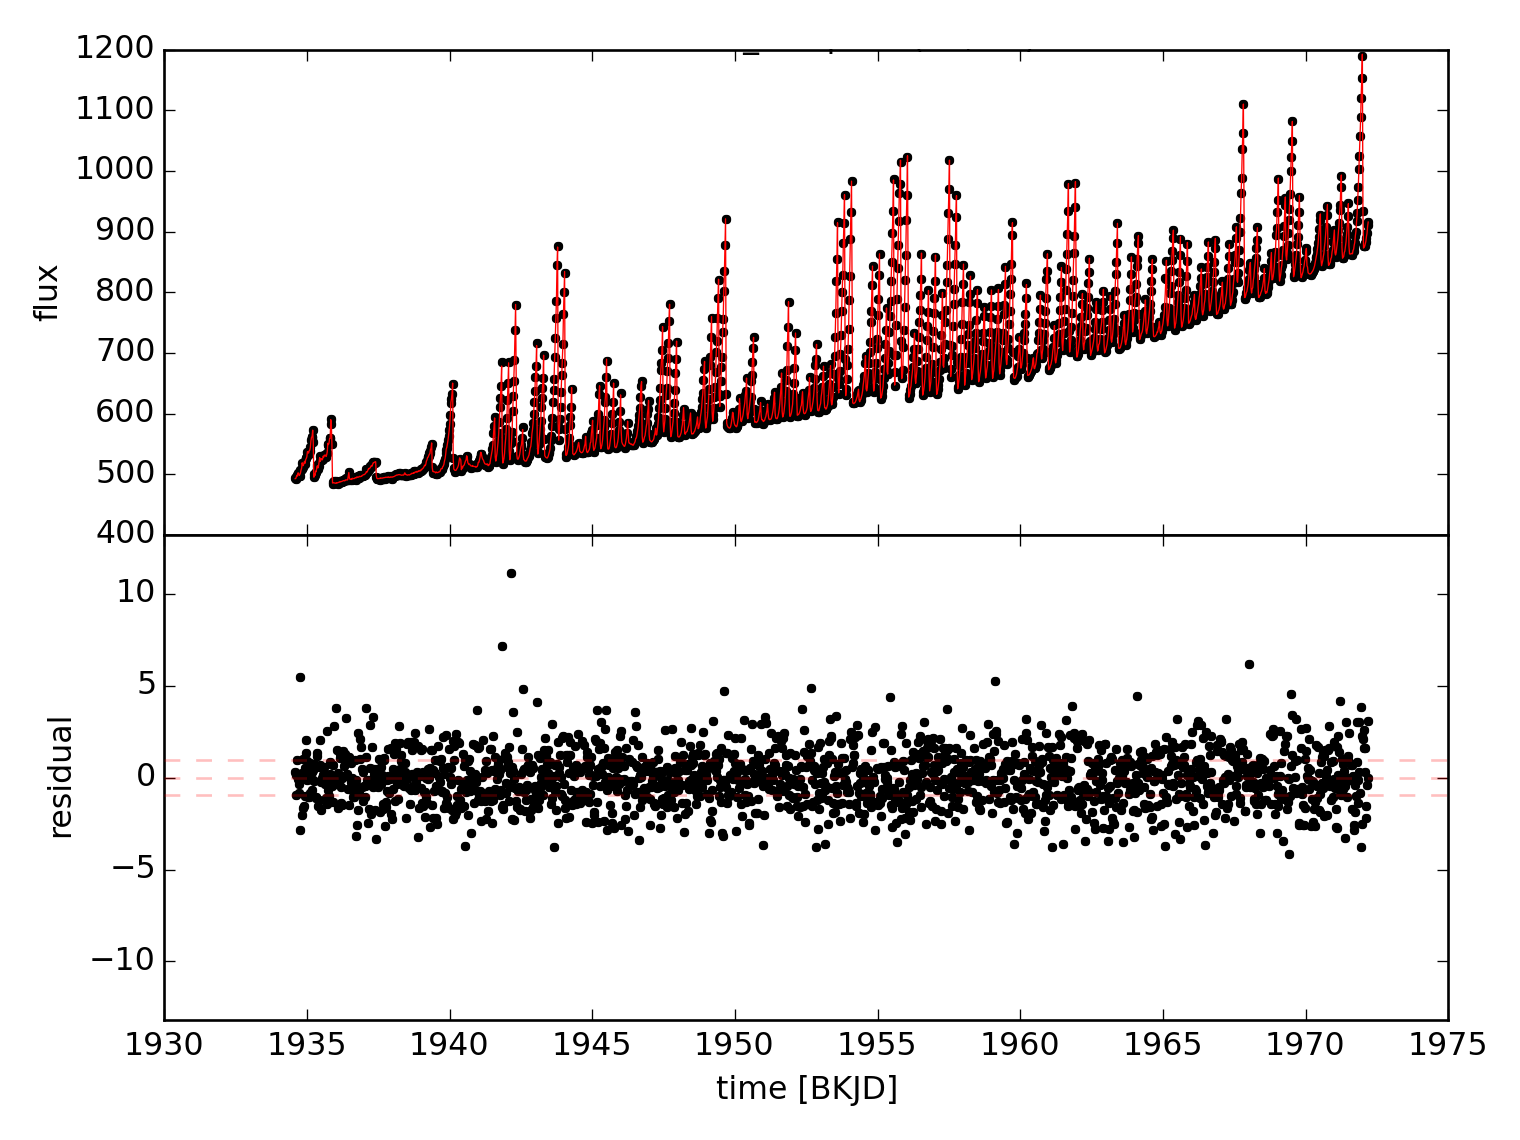
\includegraphics[width=0.95\textwidth]{f1a}
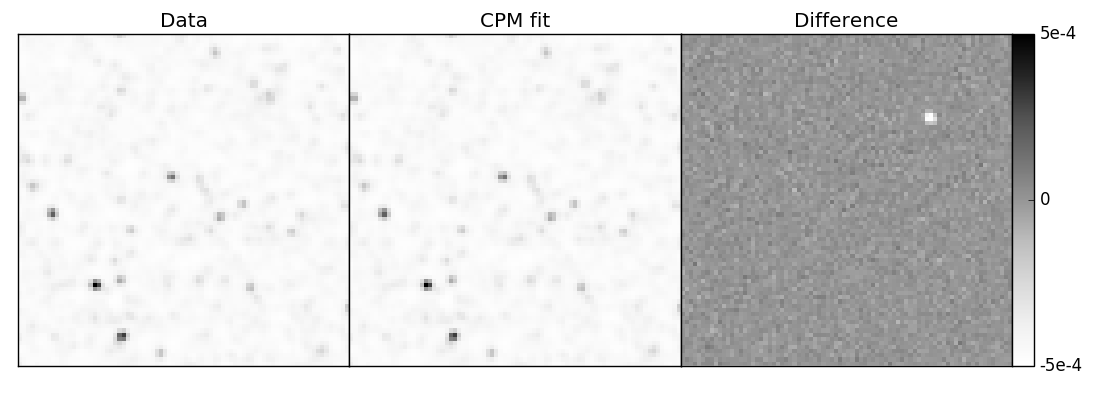
\includegraphics[width=0.95\textwidth]{f1b}
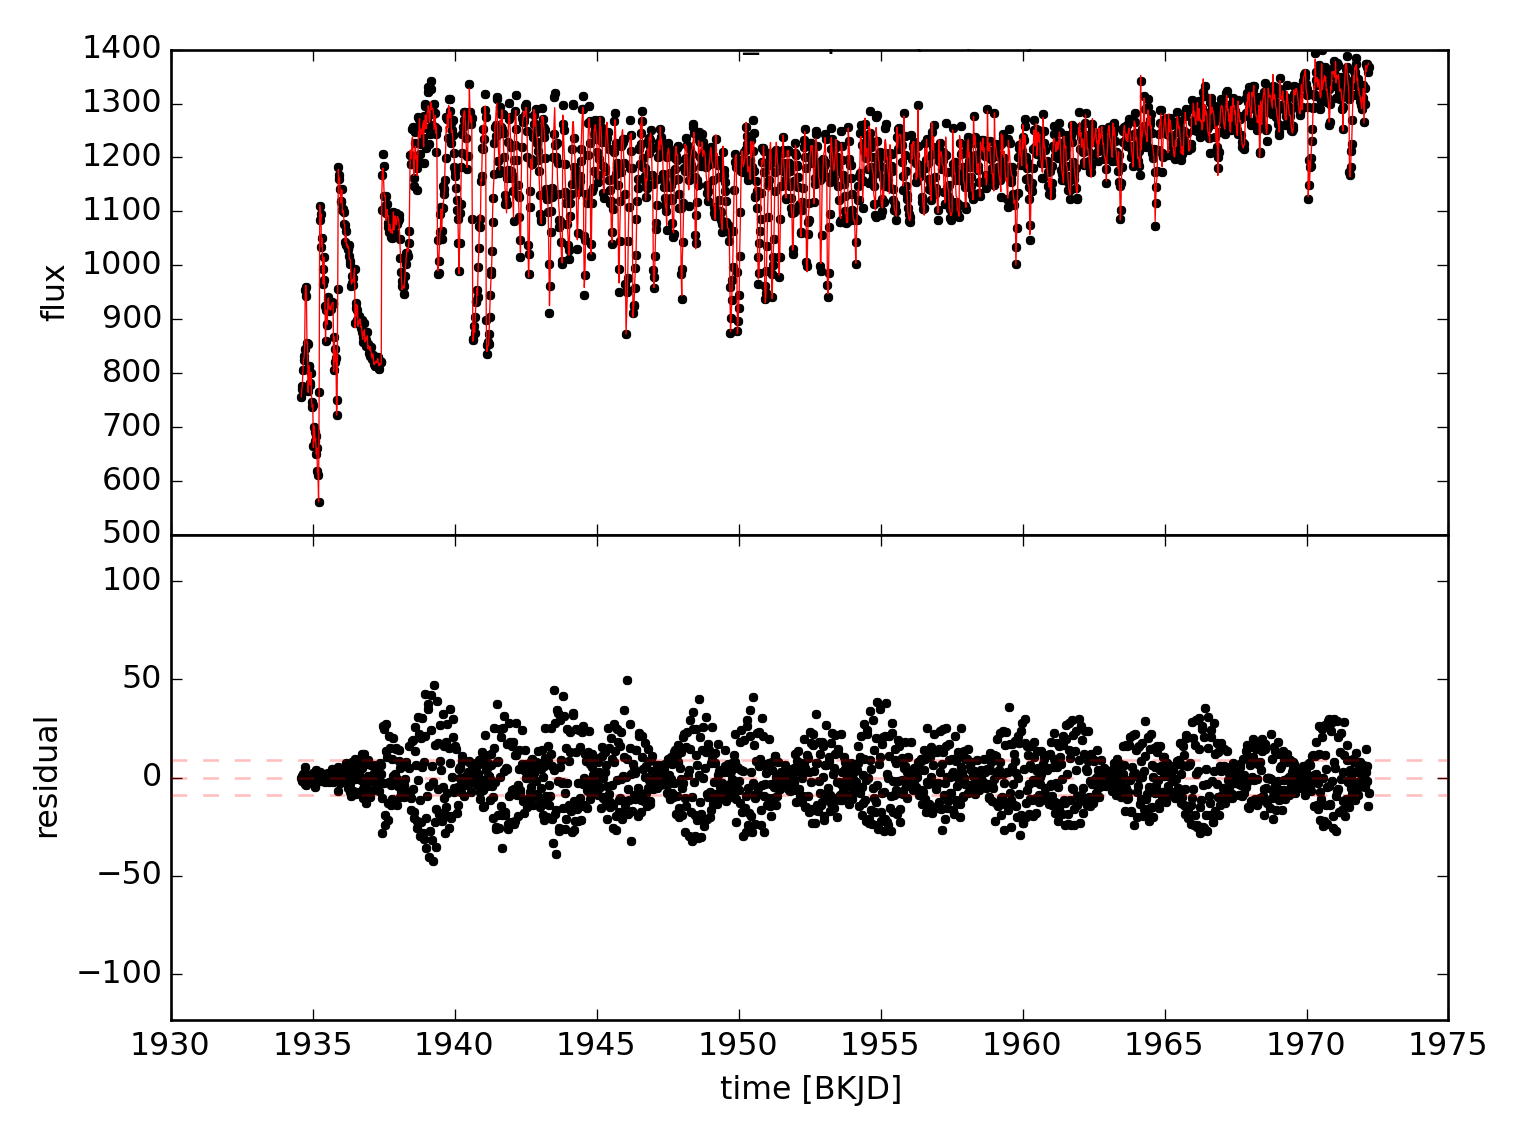
\includegraphics[width=0.95\textwidth]{f1c}
%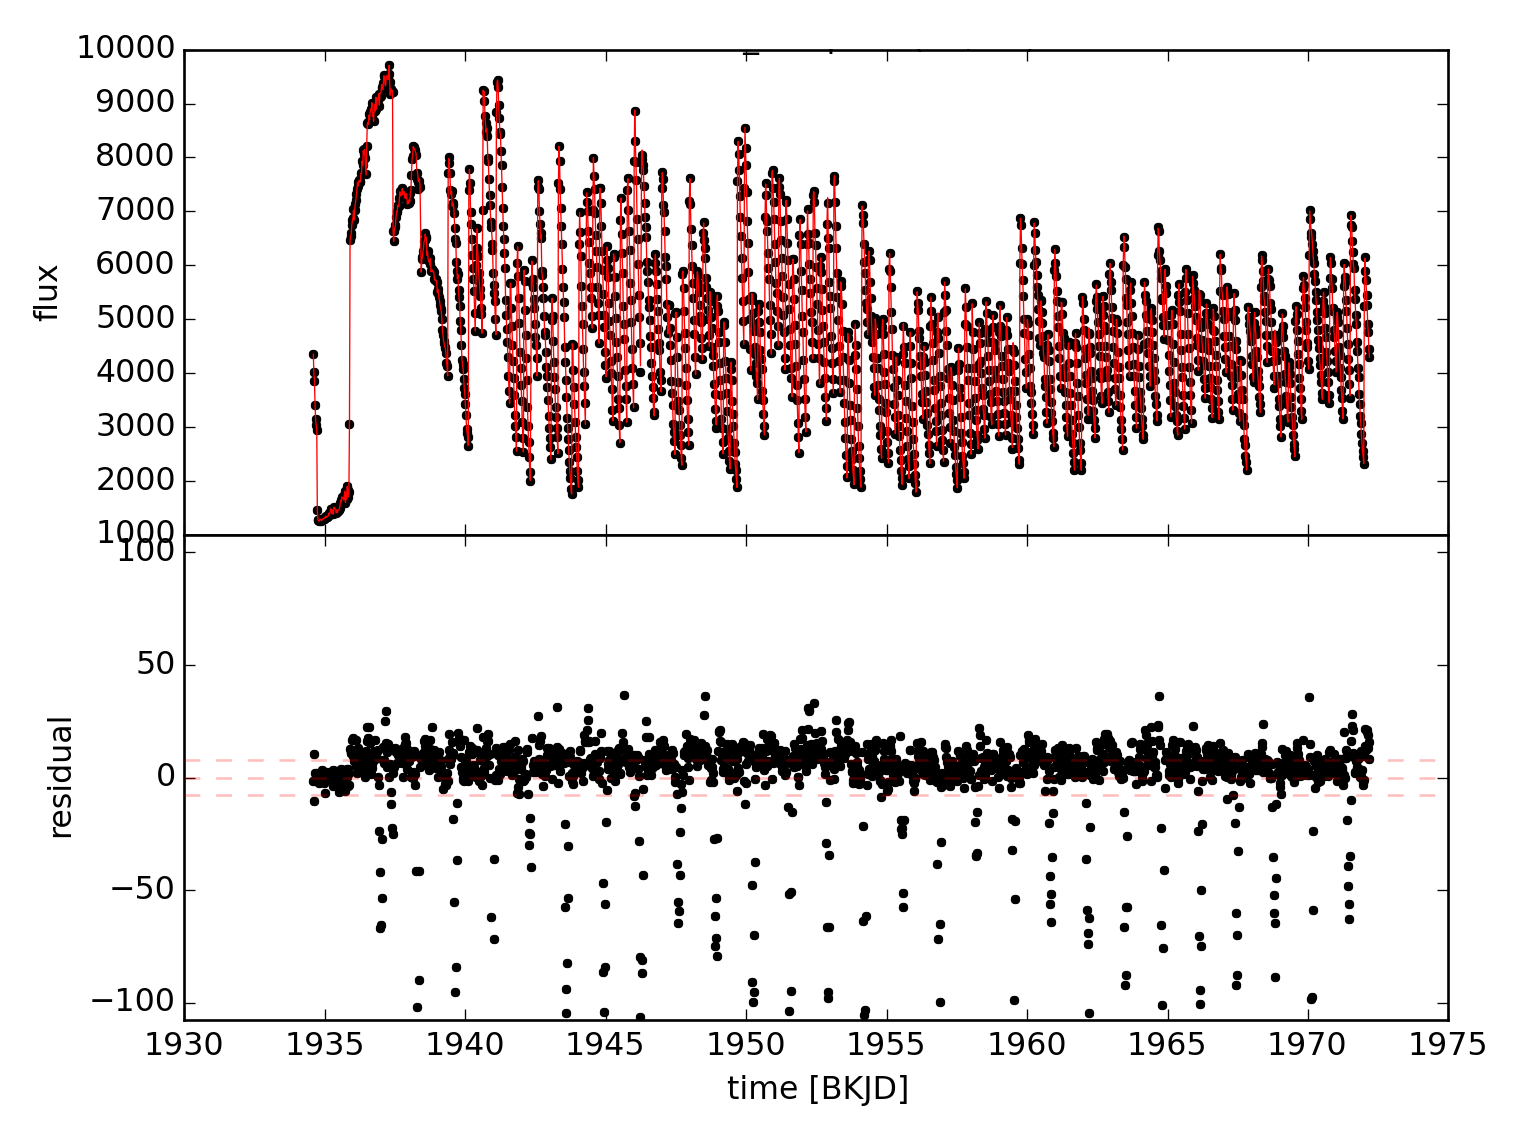
\includegraphics[width=0.95\textwidth]{f1d}
\end{center}
\caption{
  \label{space}
  An $80\times 80$ pixel mock data image patch with pointing motion. 
  From top to the bottom,  each row shows a snapshot from different times.
  \emph{Left:} mock data image;
  \emph{Middle:} the prediction of the \cpmdiff;
  \emph{Right:} the relative difference between the data and the prediction, the color bar shows the relative difference;
  Most of the pixel values are around zero, except for the varible source (upper-left corner), which means the \cpmdiff\ can predict the image data, while detects the varibles.
}
\end{figure}

\subsection{Ground-based mock data}
In ground-based observations, apart from pointing motion, weather changes and atmospheric distortions will also affect the PSF dramatically. 
Therefore the PSF variation was also included in the mock data. 
The pointing motion and rotation of the mock data are same as in the space-based test.
Variation of the PSF is achieved by varying the parameters a, b, c.
The full width half maximum in both direction are restricted between 2 to 4 pixels.
Fig~\ref{ground} shows the same mock data as in space-based test, but with PRF variation included.  
As in the space-based test,  the \cpmdiff\ was able to model both pointing motion and PRF variation, while still pulled out the variable star in the differencing image.
This experiment further confirms that \cpmdiff\ can calibrate both space-based and ground-based data.

\begin{figure}[p]
\begin{center}
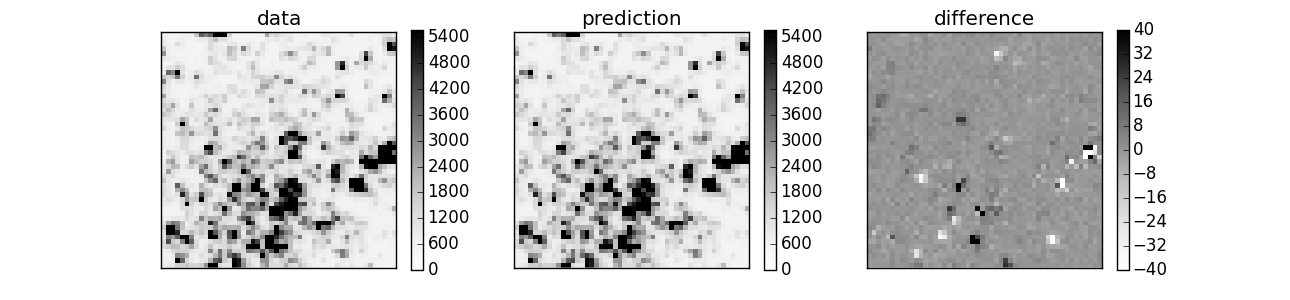
\includegraphics[width=0.95\textwidth]{f2a}
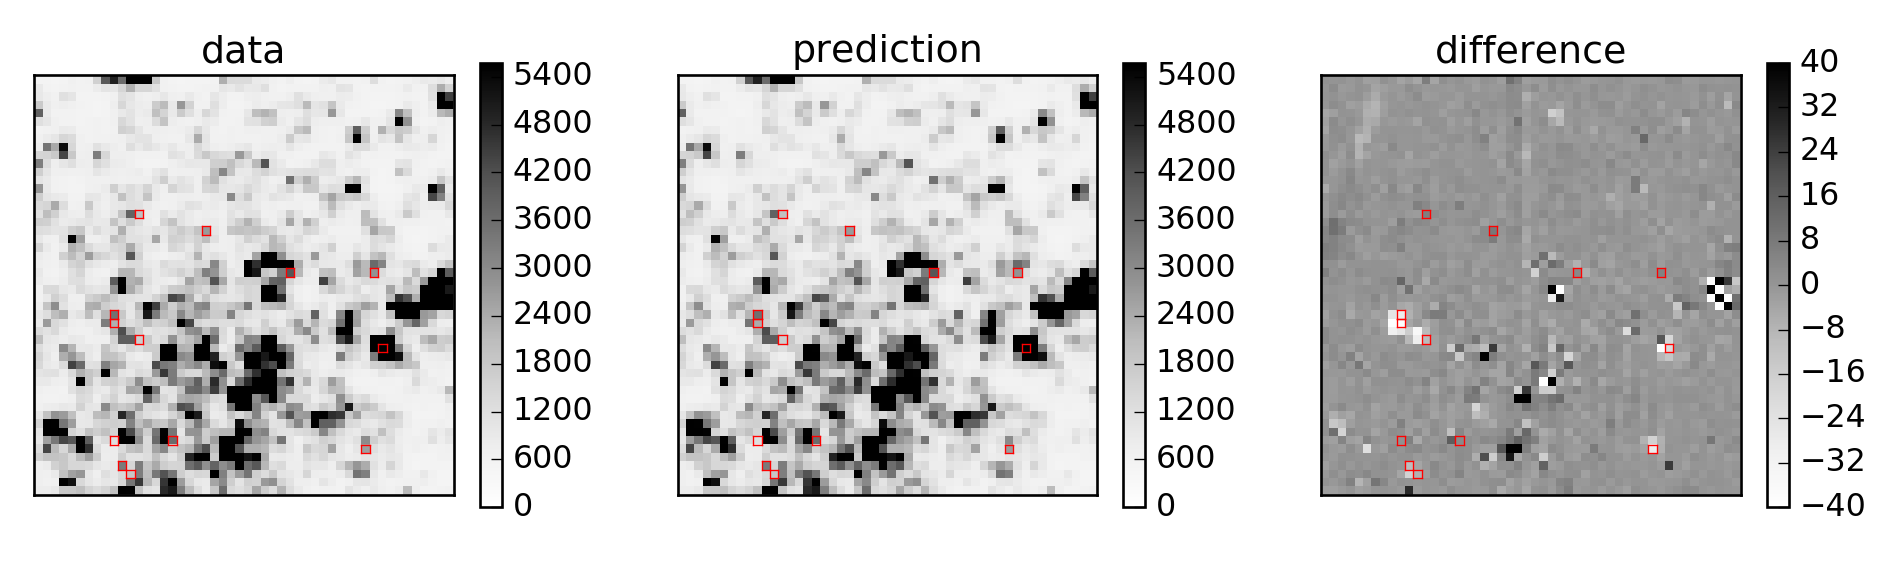
\includegraphics[width=0.95\textwidth]{f2b}
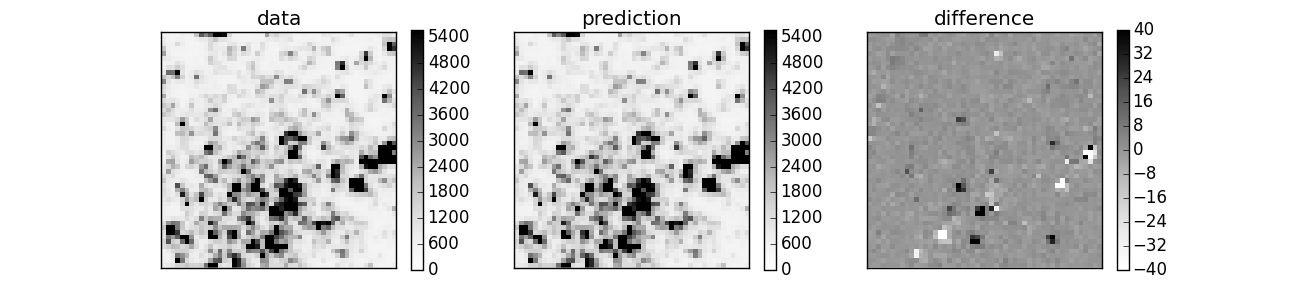
\includegraphics[width=0.95\textwidth]{f2c}
%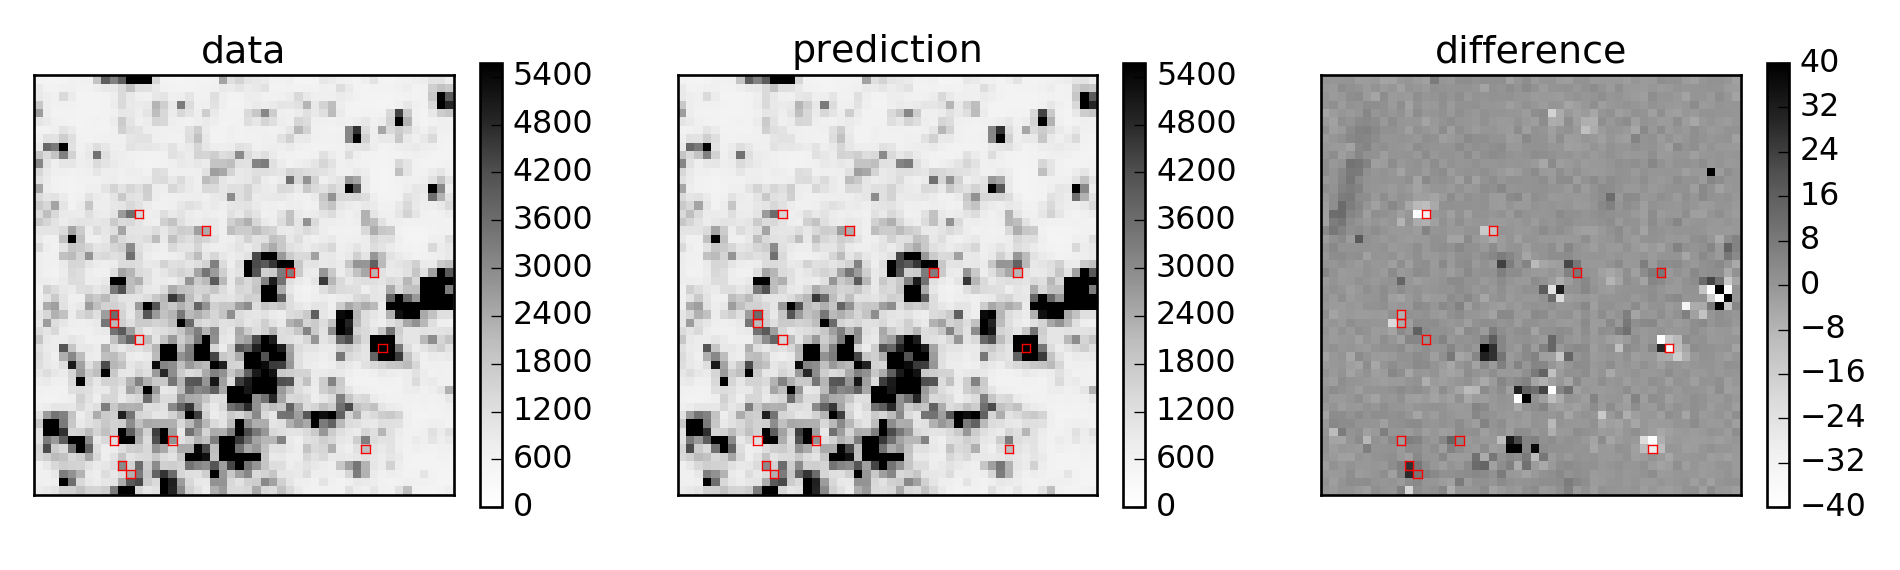
\includegraphics[width=0.95\textwidth]{f2d}
\end{center}
\caption{
  \label{ground}
  An $80\times 80$ pixel mock data image patch with both pointing motion and PRF variation. From top to the bottom,  each row shows a snapshot from different times.
  \emph{Left:} mock data image;
  \emph{Middle:} the prediction of the \cpmdiff;
  \emph{Right:} the relative difference between the data and the prediction, the color bar shows the relative difference;
  As the space-based test, \cpmdiff subtratcted all the constant stars and retained the variable sources with the ground-based mock data, which shows that the method can handle both pointing motion and PRF variation. 
}
\end{figure}

\subsection{\KTCN}
Now we test our method on a $64\times50$ pixel patch (\epic\ 200069960) from \KTCN\footnote{\url{https://keplerscience.arc.nasa.gov/k2-c9.html}}, which was dedicated to a study of gravitational microlensing events.
This data set is an ideal test bed for difference imaging, since it observed a very crowded field near the bulge, where high precision photometry is difficult to achieve directly.

Fig~\ref{k2c9} shows three snapshots of the data and the \cpmdiff\ of different times.
Constant sources in the dense field were almost all cancelled with the \cpm\ prediction, while variables (located at the red box) were preserved and can even be picked by eye from the difference image.
Variable sources were detected with the variation map (mean of absolute normalized deviations of the difference image). 
Light curves of six variable sources with highest signal to noise ratio is presented in Fig~\ref{lightcurve} as examples. 
Each light curve was constructed with simple aperture photometry, by co-adding all the difference flux within a $3 \times 3$ aperture. Note that this is not optimal photometry; it is simply illustration of what is possible.

\begin{figure}[p]
\begin{center}
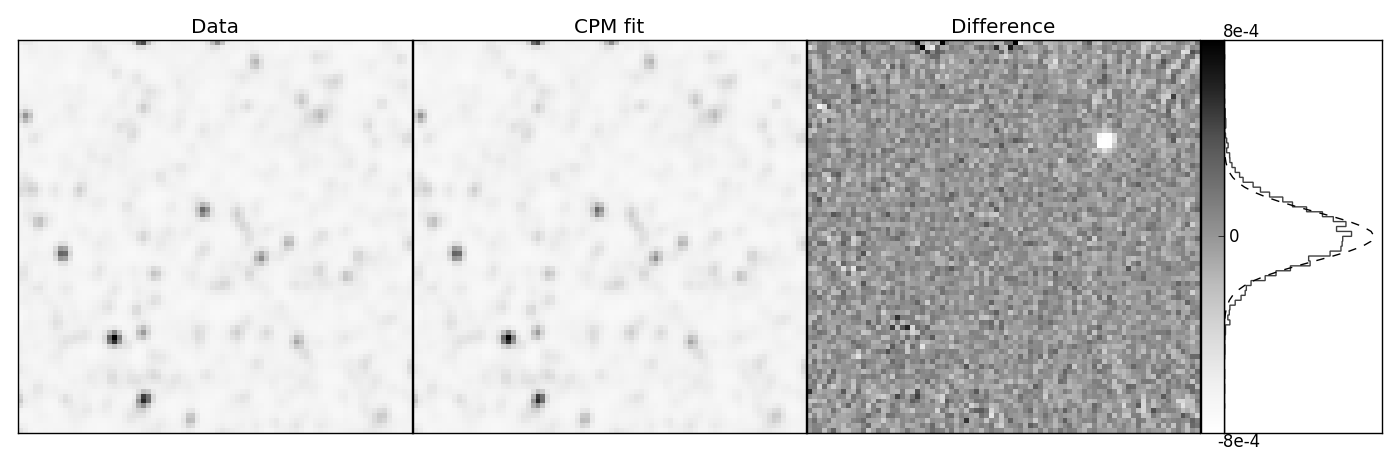
\includegraphics[width=0.95\textwidth]{f3a}
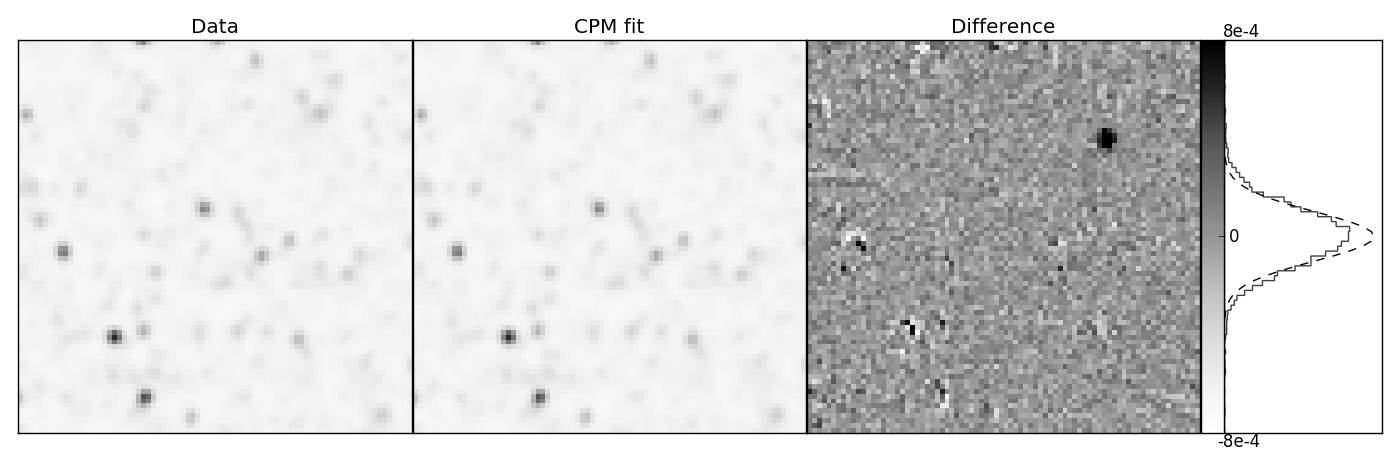
\includegraphics[width=0.95\textwidth]{f3b}
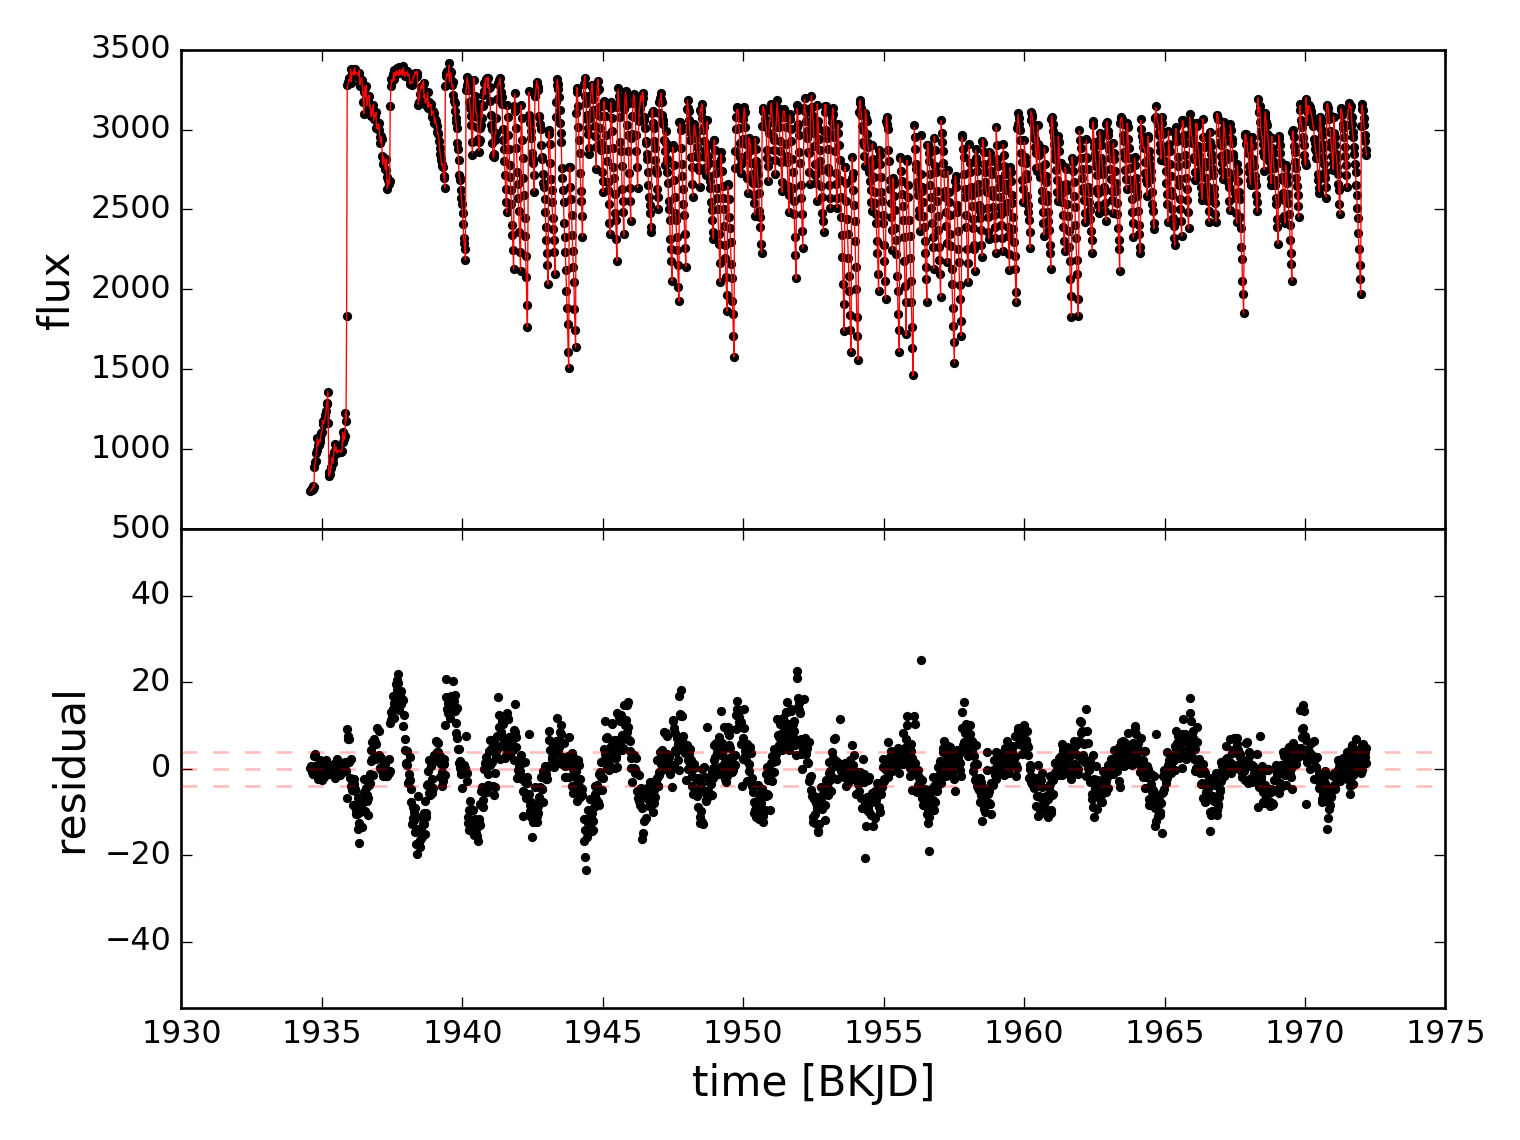
\includegraphics[width=0.95\textwidth]{f3c}
%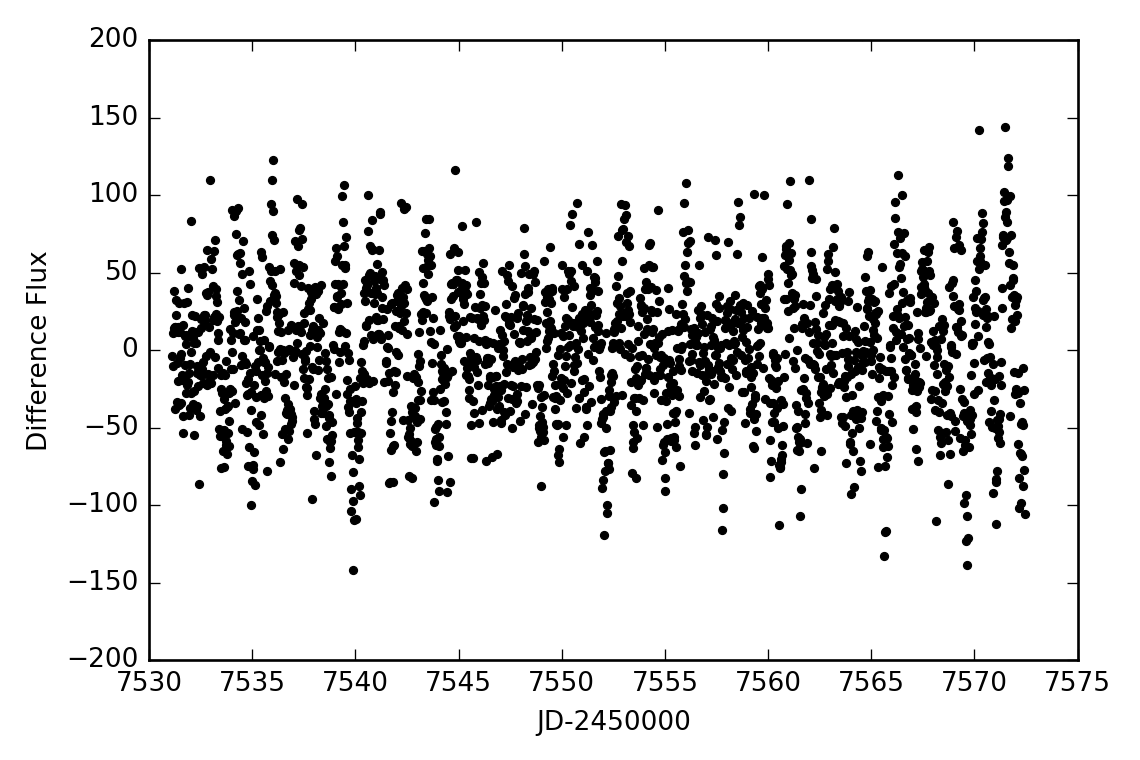
\includegraphics[width=0.95\textwidth]{f4d}
\end{center}
\caption{
  \label{k2c9}
  A $64\times 50$ pixel image patch from \KTCN\ (\epic\ 200069960). From top to the bottom,  each row shows a snapshot from different times.
  \emph{Left:} data image;
  \emph{Middle:} the prediction of the \cpmdiff;
  \emph{Right:} the difference between the data and the prediction, red boxes indicates detected variable sources.  
  The \cpmdiff\ subtracted all the constant sources in the data image, while preserve the variable sources in the difference image.
}
\end{figure}

\begin{figure}[p]
\begin{center}
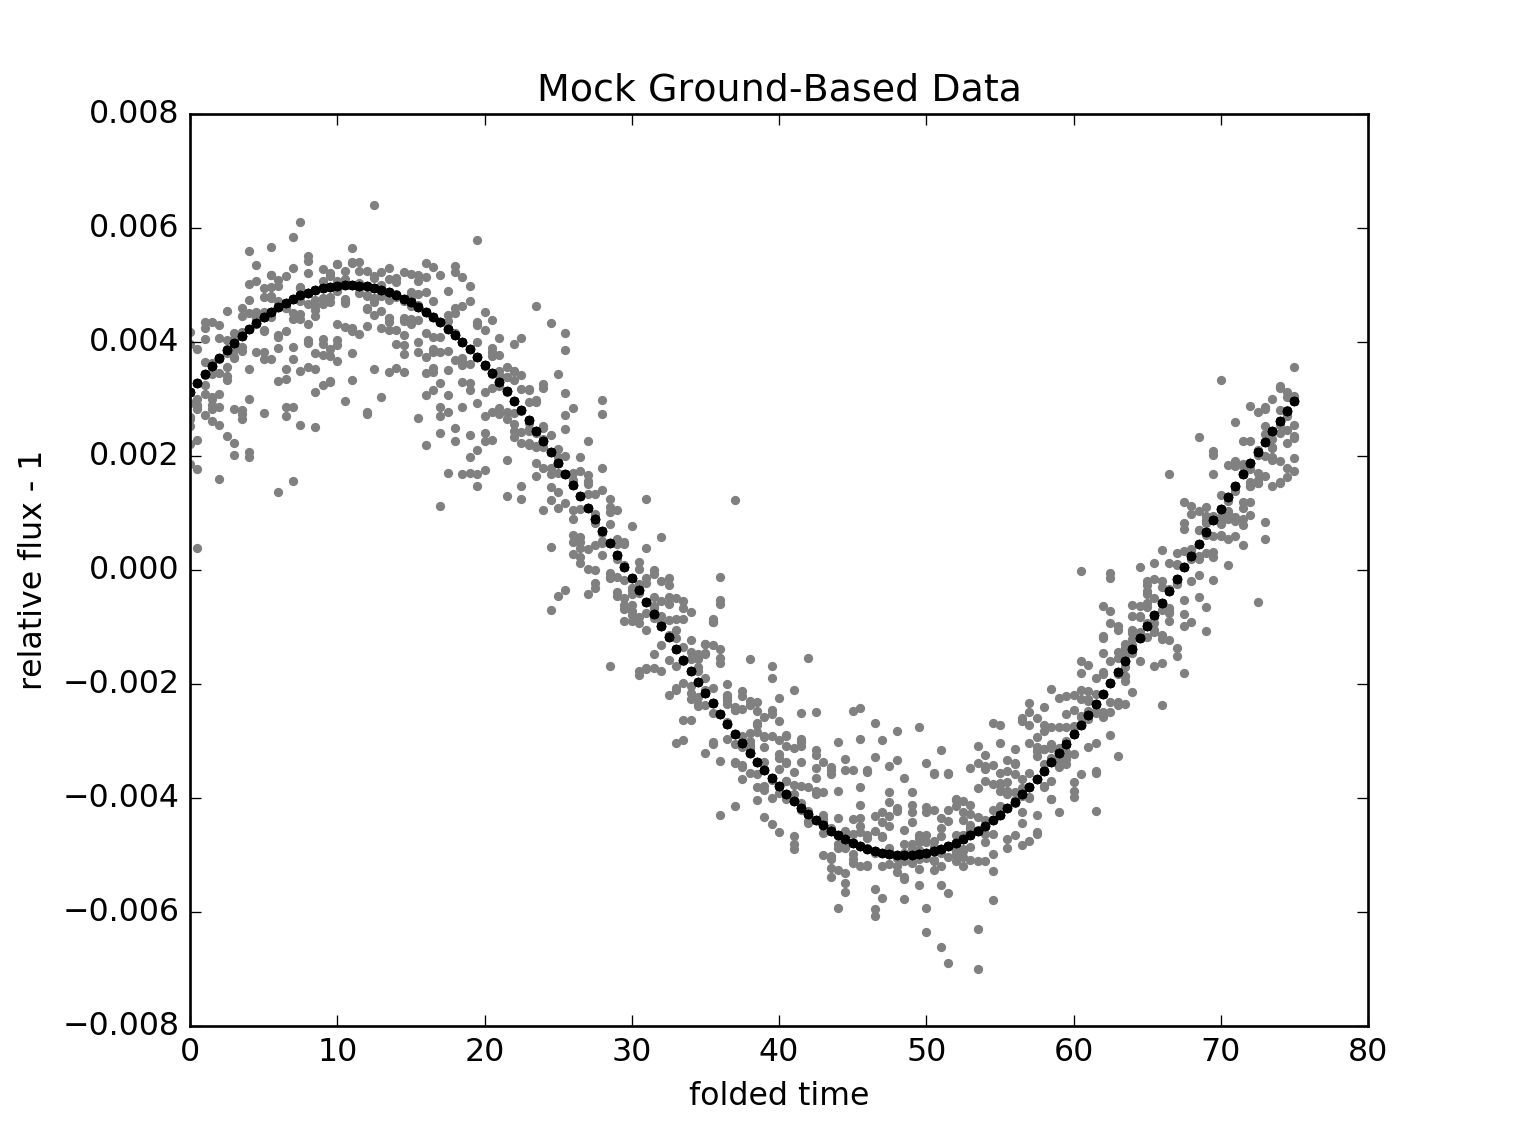
\includegraphics[width=0.48\textwidth]{f4a}
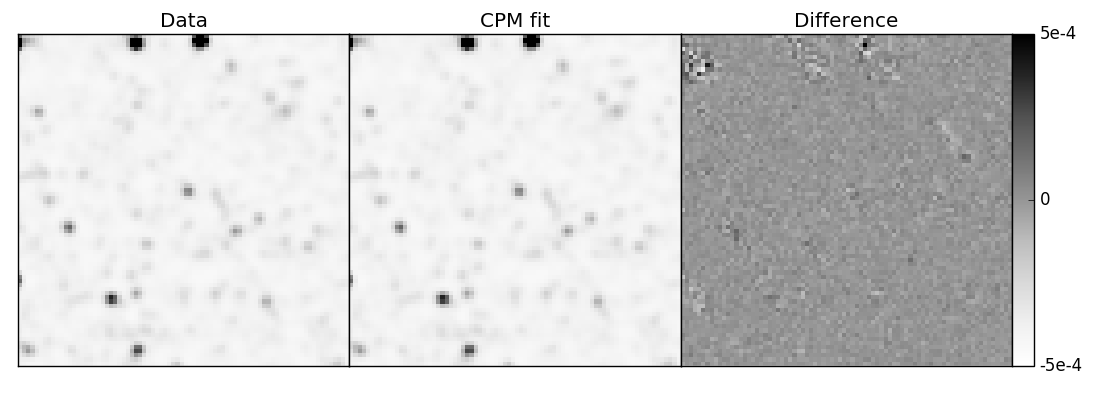
\includegraphics[width=0.48\textwidth]{f4b}
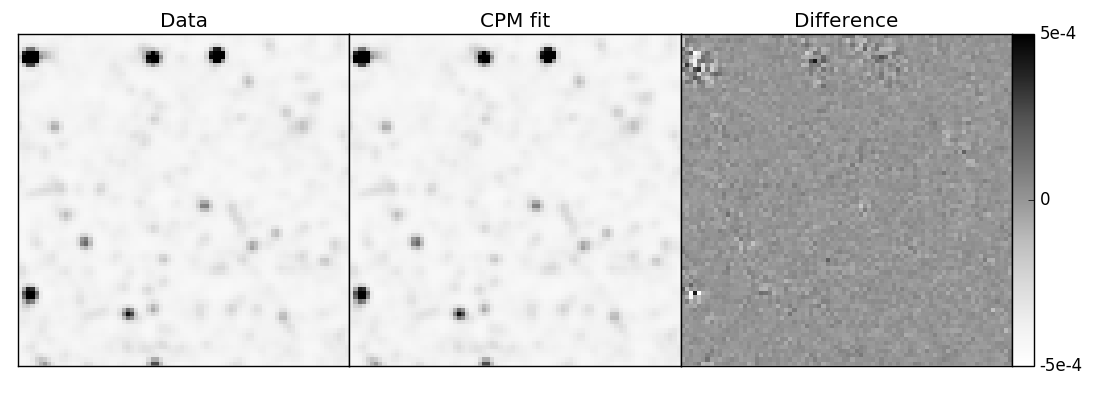
\includegraphics[width=0.48\textwidth]{f4c}
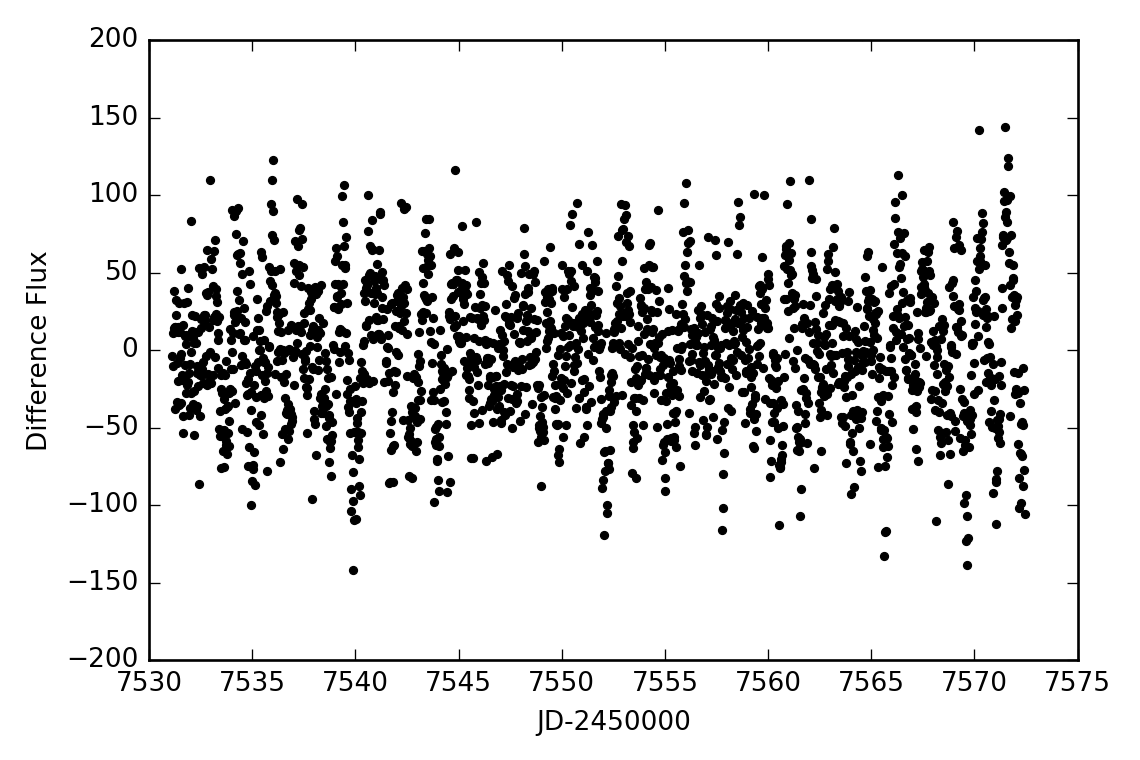
\includegraphics[width=0.48\textwidth]{f4d}
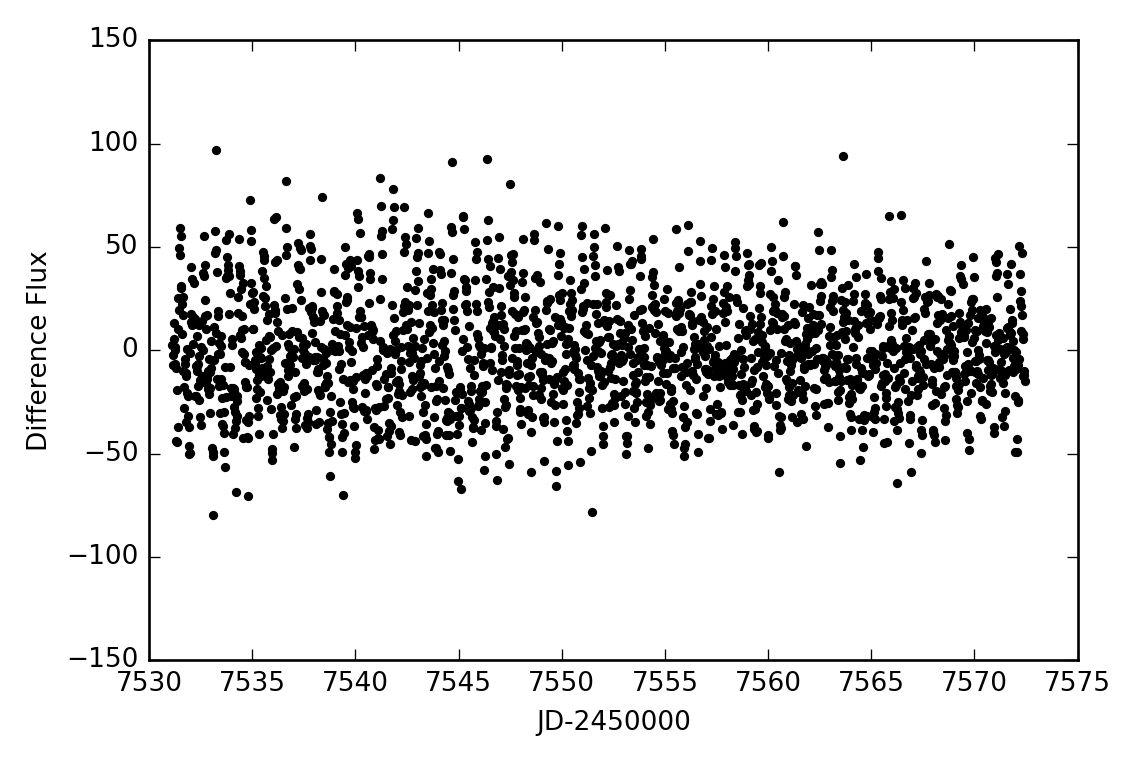
\includegraphics[width=0.48\textwidth]{f4e}
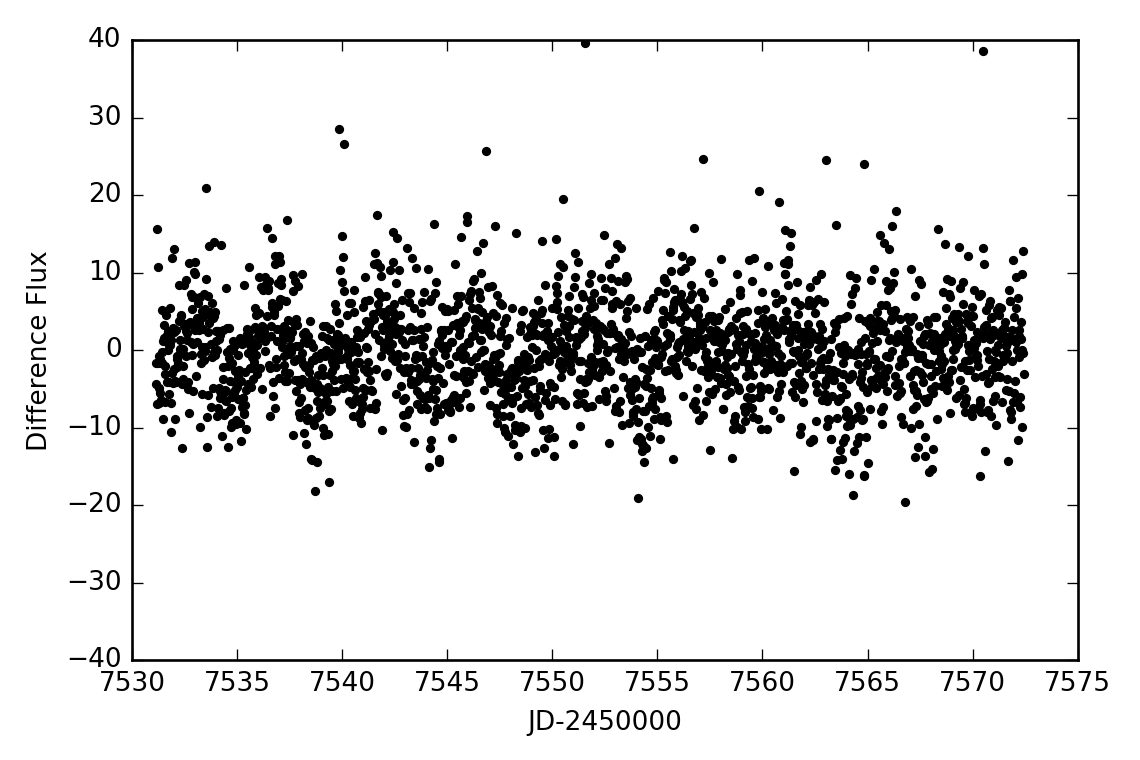
\includegraphics[width=0.48\textwidth]{f4f}
\end{center}
\caption{
  \label{lightcurve}
  Six light curves extracted from \KTCN\ \epic\ 200069960 by \cpmdiff. 
  Each light curve was generated by co-adding all the difference flux within a $3\times 3$ aperature.
}
\end{figure}


\subsection{Limitation of \cpmdiff}
In previous sections,  \cpmdiff\ was proved on both mock and real data that the method is able to model both pointing motion and PSF variations, with which variable sources detection and photometry can be achieved.
In this section, we want to push these variations to the limitation of \cpmdiff\ to define the scope of applicability of the method. Three experiments are conducted with large variations in pointing, roll and PSF.

First, overall translation up to 10 pixels was applied to the mock data to simulate the huge pointing motion.   
Fig~\ref{large_motion} shows that with large pointing motion, there is sudden jump in pixel value between image frames. 
The quality of the difference image degrades dramatically around relatively bright sources, because of the additional variabilities introduced by the motion of bright sources.
In addition,  the variable source flux also distributes in a large range of pixels due to the pointing motion, which increase the difficulties of photometric measurement.
With the same data set, in Fig~\ref{large_rotation}, the image was rotated with respect to the center up to 20 deg. 
The corner of the difference image contains large variability, since the images are worse aligned in the corner due to the rotation. 
These two test confirms the assumption that the \cpmdiff\ needs to be applied to the data set with relatively good registration.
In Fig~\ref{large_prf}, dramatic PSF variation was introduced into the mock data.
The \cpmdiff\ is able to subtract most of the constant sources even with large PSF variation. 
However with PSF varying, the distribution of the variable source flux (upper-right corner) keep changing, which makes it hard to define optimal aperture to achieve high precision photometry. 

\begin{figure}[p]
\begin{center}
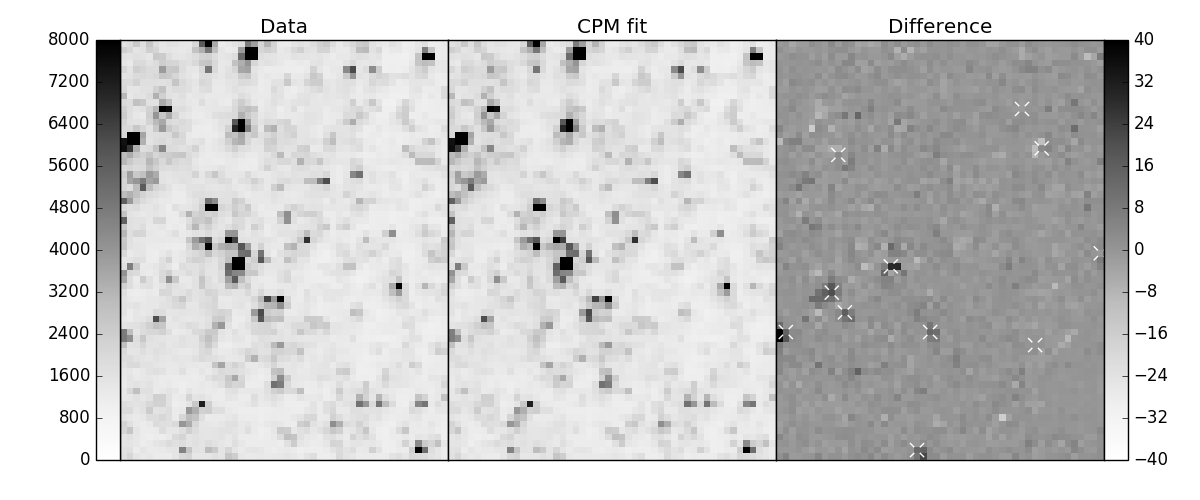
\includegraphics[width=0.95\textwidth]{f5a}
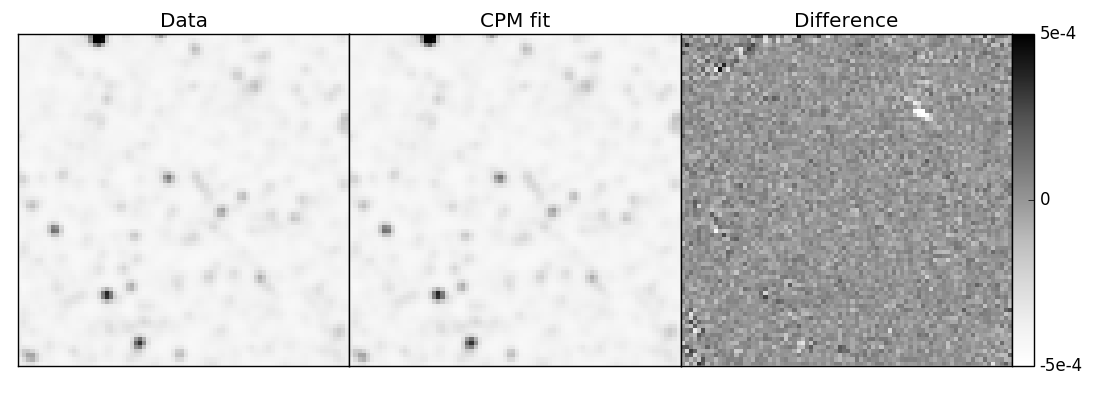
\includegraphics[width=0.95\textwidth]{f5b}
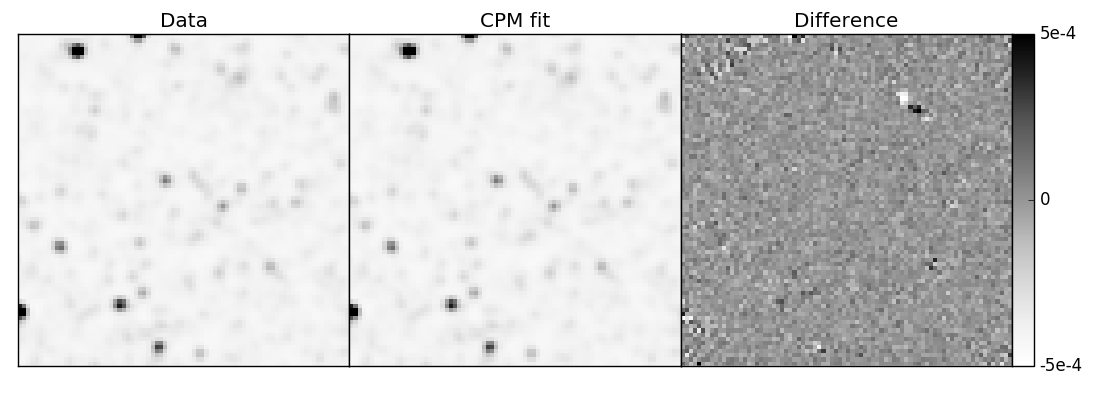
\includegraphics[width=0.95\textwidth]{f5c}
%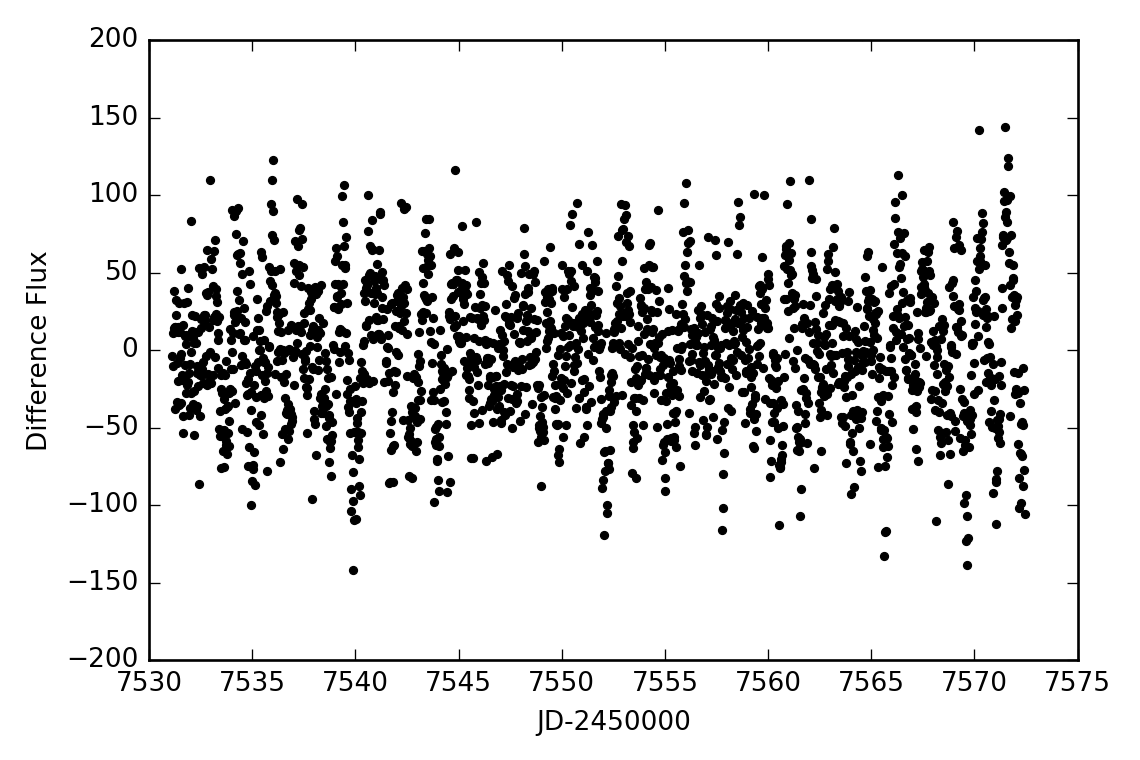
\includegraphics[width=0.95\textwidth]{f4d}
\end{center}
\caption{
  \label{large_motion}
  An $80\times 80$ pixel mock data image patch with overall translation up to 10 pixels. From top to the bottom,  each row shows a snapshot from different times.
  \emph{Left:} mock data image;
  \emph{Middle:} the prediction of the \cpmdiff;
  \emph{Right:} the relative difference between the data and the prediction; 
  Additional variabilities are introduced into the difference image by motion of bright sources.
}
\end{figure}


\begin{figure}[p]
\begin{center}
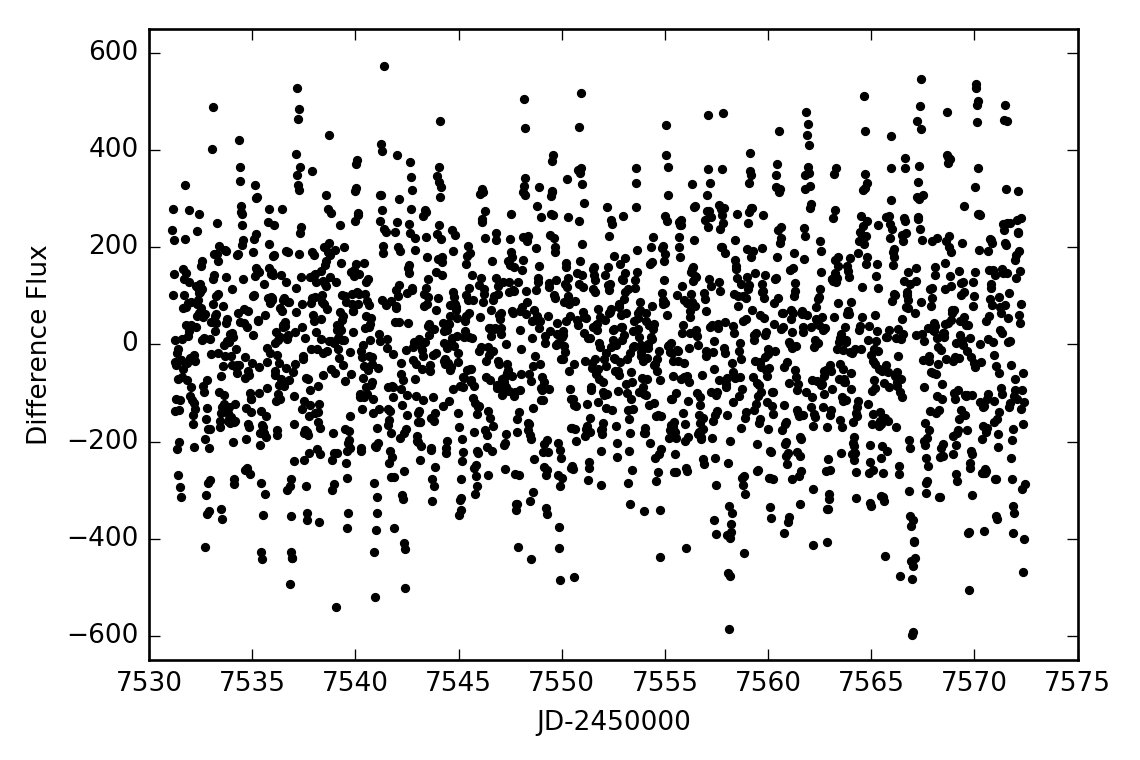
\includegraphics[width=0.95\textwidth]{f6a}
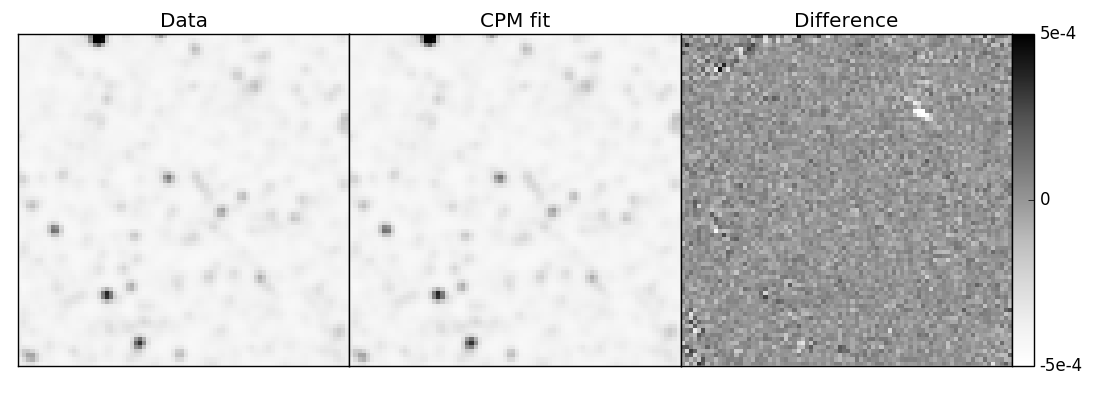
\includegraphics[width=0.95\textwidth]{f6b}
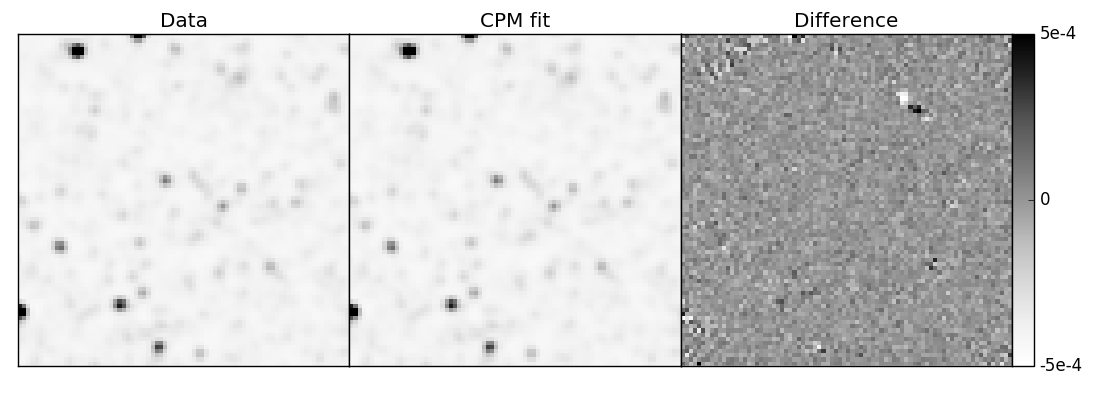
\includegraphics[width=0.95\textwidth]{f6c}
%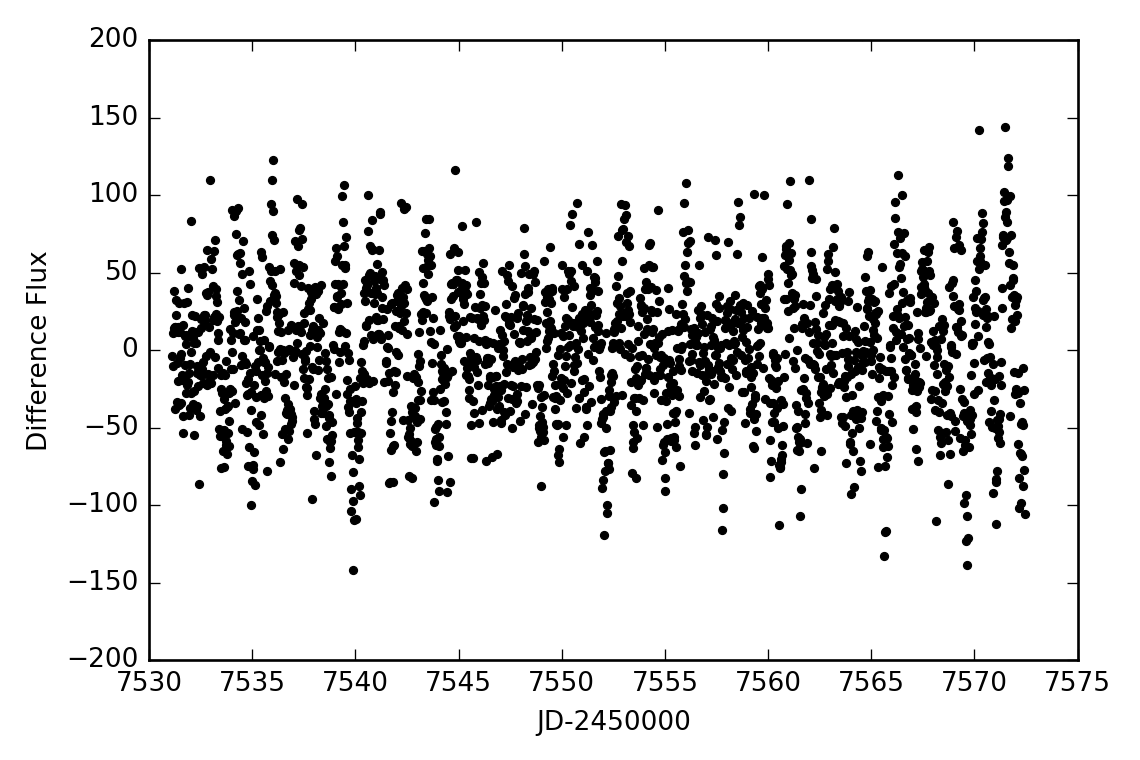
\includegraphics[width=0.95\textwidth]{f4d}
\end{center}
\caption{
  \label{large_rotation}
  An $80\times 80$ pixel mock data image patch with rotation up to 20 deg. 
  From top to the bottom, each row shows a snapshot from different times.
  \emph{Left:} mock data image;
  \emph{Middle:} the prediction of the \cpmdiff;
  \emph{Right:} the relative difference between the data and the prediction;
  The quality of the difference image drops dramtically in the corner due to the rotaion.   
}
\end{figure}

\begin{figure}[p]
\begin{center}
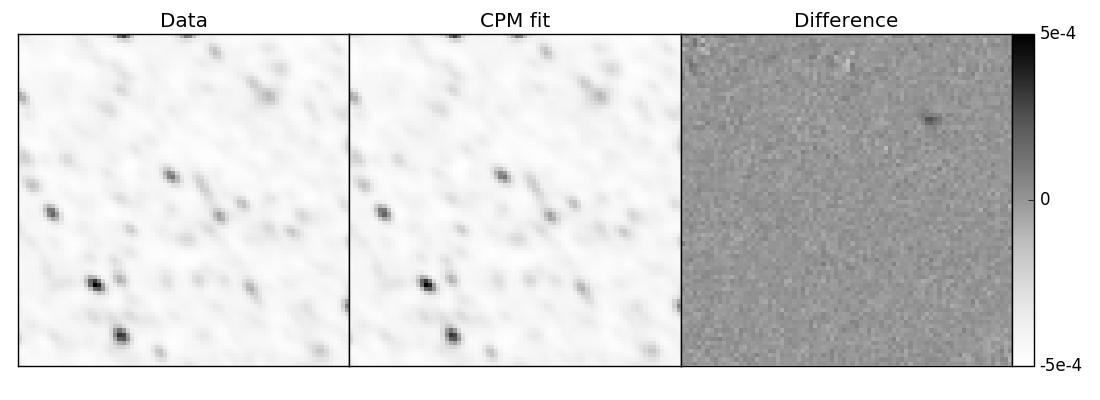
\includegraphics[width=0.95\textwidth]{f7a}
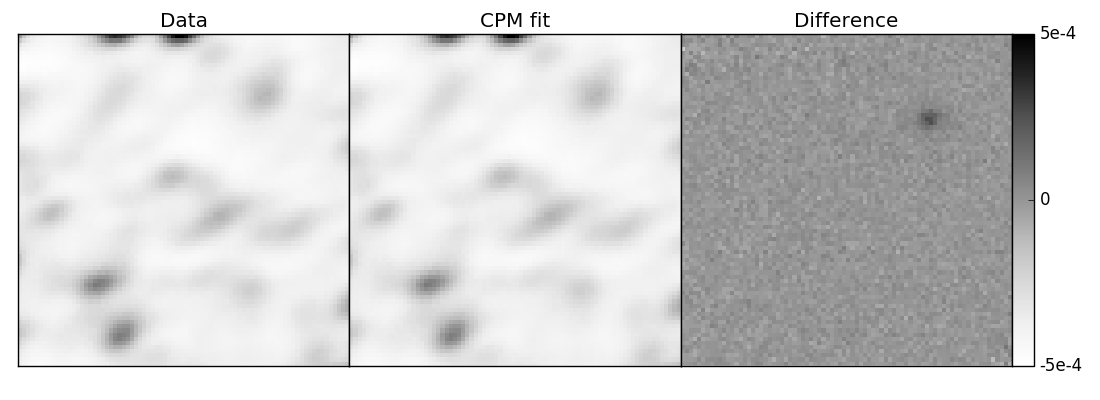
\includegraphics[width=0.95\textwidth]{f7b}
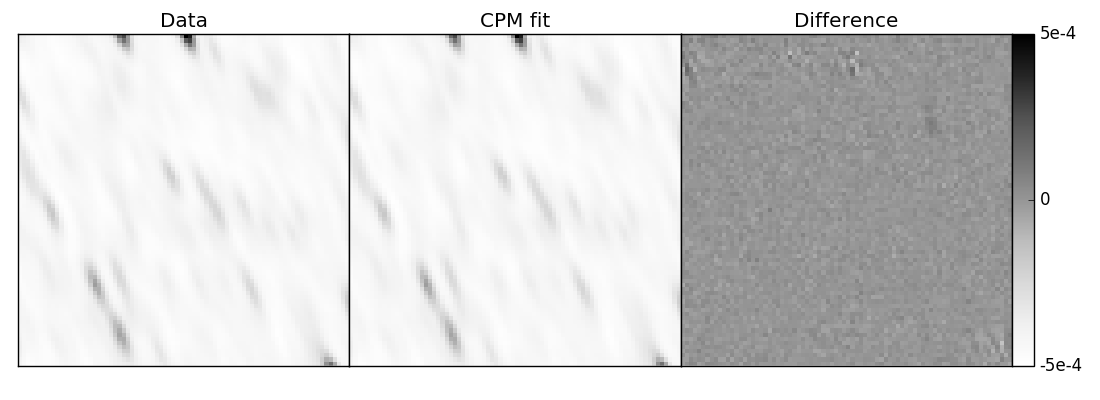
\includegraphics[width=0.95\textwidth]{f7c}
%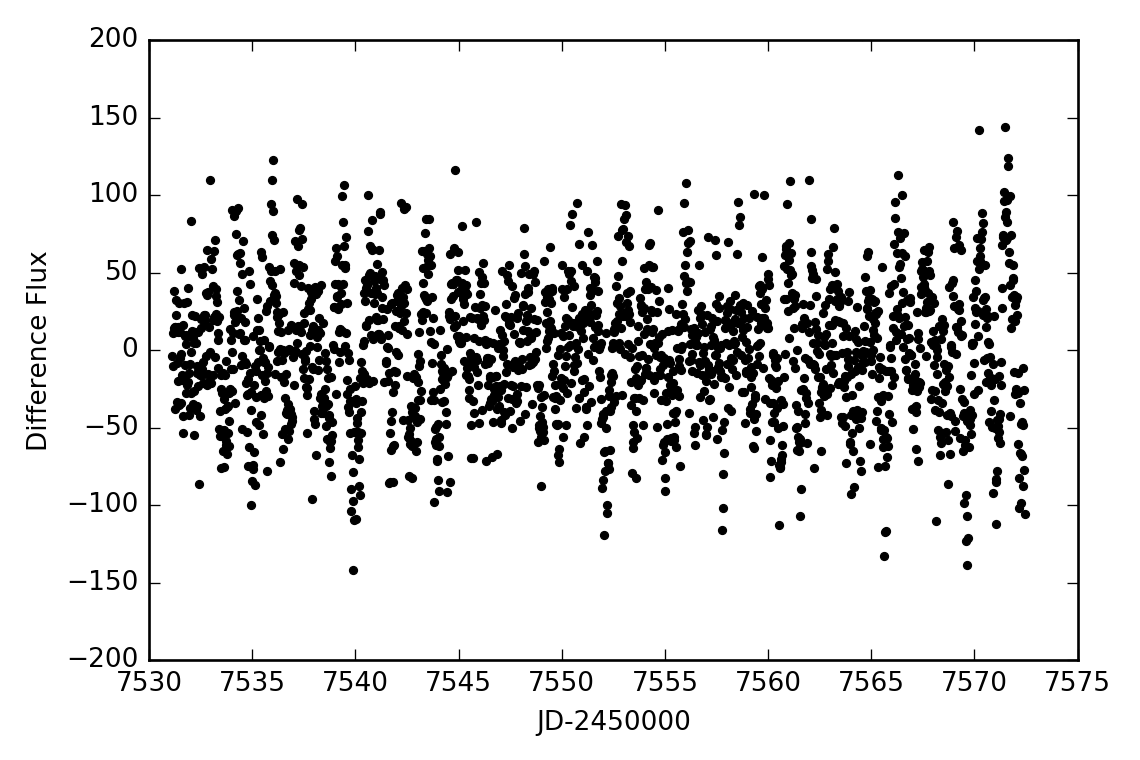
\includegraphics[width=0.95\textwidth]{f4d}
\end{center}
\caption{
  \label{large_prf}
  An $80\times 80$ pixel mock data image patch with large PSF variation. 
  From top to the bottom, each row shows a snapshot from different times.
  \emph{Left:} mock data image;
  \emph{Middle:} the prediction of the \cpmdiff;
  \emph{Right:} the relative difference between the data and the prediction;  
  \cpmdiff\ is able to subtract images with huge PSF variation. 
  However the distribution of the varible source flux also changes dramtically with the PSF variation, which increase difficulty to achieve high precision photomerty.
}
\end{figure}





\section{Discussion}
\todo{data taken differently}

\clearpage
\bibliography{cdi}
\clearpage

\end{document}